%!TeX program=pdflatex
\documentclass[titlepage]{article}
 
\usepackage[margin=1in]{geometry} 
\usepackage{amsmath,amsthm,amssymb,fancyhdr,gensymb,arydshln,graphicx}
\graphicspath{{C:/Users/user/Desktop/}}

\pagestyle{fancy}

\newenvironment{theorem}[2][Theorem]{\begin{trivlist}
\item[\hskip \labelsep {\bfseries #1}\hskip \labelsep {\bfseries #2.}]}{\end{trivlist}}
\newenvironment{lemma}[2][Lemma]{\begin{trivlist}
\item[\hskip \labelsep {\bfseries #1}\hskip \labelsep {\bfseries #2.}]}{\end{trivlist}}
\newenvironment{exercise}[2][Exercise]{\begin{trivlist}
\item[\hskip \labelsep {\bfseries #1}\hskip \labelsep {\bfseries #2.}]}{\end{trivlist}}
\newenvironment{problem}[2][Problem]{\begin{trivlist}
\item[\hskip \labelsep {\bfseries #1}\hskip \labelsep {\bfseries #2.}]}{\end{trivlist}}
\newenvironment{question}[2][Question]{\begin{trivlist}
\item[\hskip \labelsep {\bfseries #1}\hskip \labelsep {\bfseries #2.}]}{\end{trivlist}}
\newenvironment{corollary}[2][Corollary]{\begin{trivlist}
\item[\hskip \labelsep {\bfseries #1}\hskip \labelsep {\bfseries #2.}]}{\end{trivlist}}


\begin{document}
 
% --------------------------------------------------------------
%                         Start here
% --------------------------------------------------------------
 
%\title{Weekly Homework II}%replace X with the appropriate number
%\author{Dakota Wicker\\ %replace with your name
%Abstract Algebra I} %if necessary, replace with your course title
%\maketitle
%\clearpage
\fancyhf{}
\fancyhead[RO,RE]{Abstract I}
\fancyhead[LO,LE]{Dakota Wicker}
\fancyhead[CO,CE]{Homework IV}
\cfoot{\thepage}

\begin{problem}{1}
Let
$$ S = \{A \in M_n(\mathbb{R}) | \det(A) = 7^k \ \text{for some integer }k\}. $$
\begin{itemize}
\item[(a)] Use Corollary 4.2.2 to prove that $S \leq GL(n,\mathbb{R})$.
\item[(b)] Use Corollary 4.2.3 to prove that $S \leq GL(n,\mathbb{R})$.
\end{itemize}
\hrulefill
\begin{itemize}
\item[(a)] \begin{proof}
$S$ is a nonempty set because when $k=0$, the identity matrix, $I \in S$ because $\det(I) = 1 = 7^0$ and $I^{-1} = I$. $S$ is closed under multiplication in $GL(n,\mathbb{R})$ because matrix multiplication is known to be closed and since $\det(AB) = \det(A)\det(B) = \det(7^a)\det(7^b) = \det(7^{a+b}),\ a,b\in\mathbb{Z} ,\ B \in S$ and $7^{a+b} \neq 0$, it follows that $AB$ is invertible and has a determinant in the form $7^k$ which means $AB \in S$. To show that an inverse exists $\forall A \in S$, I use the fact that $A\in GL(n,\mathbb{R})$, so $A$ is invertible and $\det(A^{-1}) = \frac{1}{\det(A)}$. It follows that since $A\in S, \det(A) = 7^n$, and that $\det(A^{-1}) = \frac{1}{7^n} = 7^{-n}$. Since $A^{-1}$ exists and has a determinant in the form of $7^k$, $A^{-1} \in S$. Since $S$ is closed under matrix multiplication and $\forall a\in S$, $a^{-1} \in S$, by Corollary 4.2.2, $S$ is a subset of $GL(n,R)$.\end{proof}

\item[(b)]\begin{proof}
$S$ is a nonempty set because when $k=0$, the identity matrix, $I \in S$ because $\det(I) = 1 = 7^0$ and $I^{-1} = I$. Since $\det(A) = 7^k$ and $\det(B^{-1}) = \frac{1}{7^n} = 7^{-n}$ where $B \in S$ and $\det(B)=7^n$, then $\det(AB^{-1}) = \det(A)\det(B^{-1}) = 7^k 7^{-n} = 7^{k-n }.$ Since $\det(AB^{-1}) = 7^{k-n}$, $AB^{-1}$ is invertible and takes the form $7^k$. Therefore $AB^{-1} \in S$. Since $AB^{-1} \in S, \ \forall A,B \in S$, this satasfies all of the conditions for Corollary 4.2.3 and therefore $S$ is a subgroup of $GH(n,\mathbb{R})$.  
\end{proof}
\end{itemize}
\end{problem}
\begin{problem}{2}
Recall that
$$ S = \left\{\begin{bmatrix}1&0\\k&1\end{bmatrix} \bigg| k \in \mathbb{Z}_{120}\right\}$$
forms a group under multiplication. Prove, in the easiest way, that
$$T = \left\{ \begin{bmatrix} 1 & 0 \\ 3k & 1 \end{bmatrix} \bigg| k \in \mathbb{Z}_{120} \right\}$$
is a subgroup of $S$.
\\
\\
Since $\forall a,b \in T$, $ab\in T$ because $\begin{bmatrix}1&0 \\ 3k & 1\end{bmatrix} \begin{bmatrix}1 & 0 \\ 3n & 1 \end{bmatrix} = \begin{bmatrix}1 & 0 \\ 3(k+n) & 1 \end{bmatrix}$ and since $ab$ takes the form $\begin{bmatrix} 1 & 0 \\ 3k & 1 \end{bmatrix}, k \in \mathbb{Z}_{120}$, this means $ab \in T$. It is also true that $\forall a \in T $, $a^{-1}$ exists. To show that $a^{-1}$ exists, I show that there is an element $a^-1$ such that $aa^{-1} = I$. If I let $n = -k$, $\begin{bmatrix}1&0 \\ 3k & 1\end{bmatrix} \begin{bmatrix}1 & 0 \\ 3n & 1 \end{bmatrix} = \begin{bmatrix}1 & 0 \\ 3(k+-k) & 1 \end{bmatrix} = \begin{bmatrix}1 & 0 \\ 3(0) & 1 \end{bmatrix} = \begin{bmatrix}1 & 0 \\ 0 & 1 \end{bmatrix} = I $ therefore the inverse is $\begin{bmatrix}1&0\\-3k&1 \end{bmatrix}$. Since $T$ is closed under $S$'s binary operation and $\forall a \in T, a^{-1}$ exists, by Corollary 4.2.2, $T$ is a subgroup of $S$.
\end{problem}

\begin{problem}{3}
Consider $D_{12}$, the dihedral group of degree 12.
\begin{itemize}
\item[(a)] List its elements using the notation we used in class.
\item[(b)] Use the geometric interpretation of the rigid transformations to explain why $$ R_{180}F_1R_{180} = F_1.$$
\item[(c)] Is it true that $R_{180}F_iF_{180} = F_i $for any i? Explain. 
\item[(d)] Is it true that $R_{180}E_iF_{180} = E_i$ for any i? Explain. 
\end{itemize}
\hrulefill \\
(a)\\$D_{12} = {R_0, R_{30},R_{60},R_{90},R_{120},R_{150},R_{180},R_{210},R_{240},R_{270},R_{300},R_{330},R_{360},F_1,F_2,F_3,F_4,F_5,F_6,E_1,E_2,E_3,E_4,E_5,E_6}$
\\ \\(b)\\

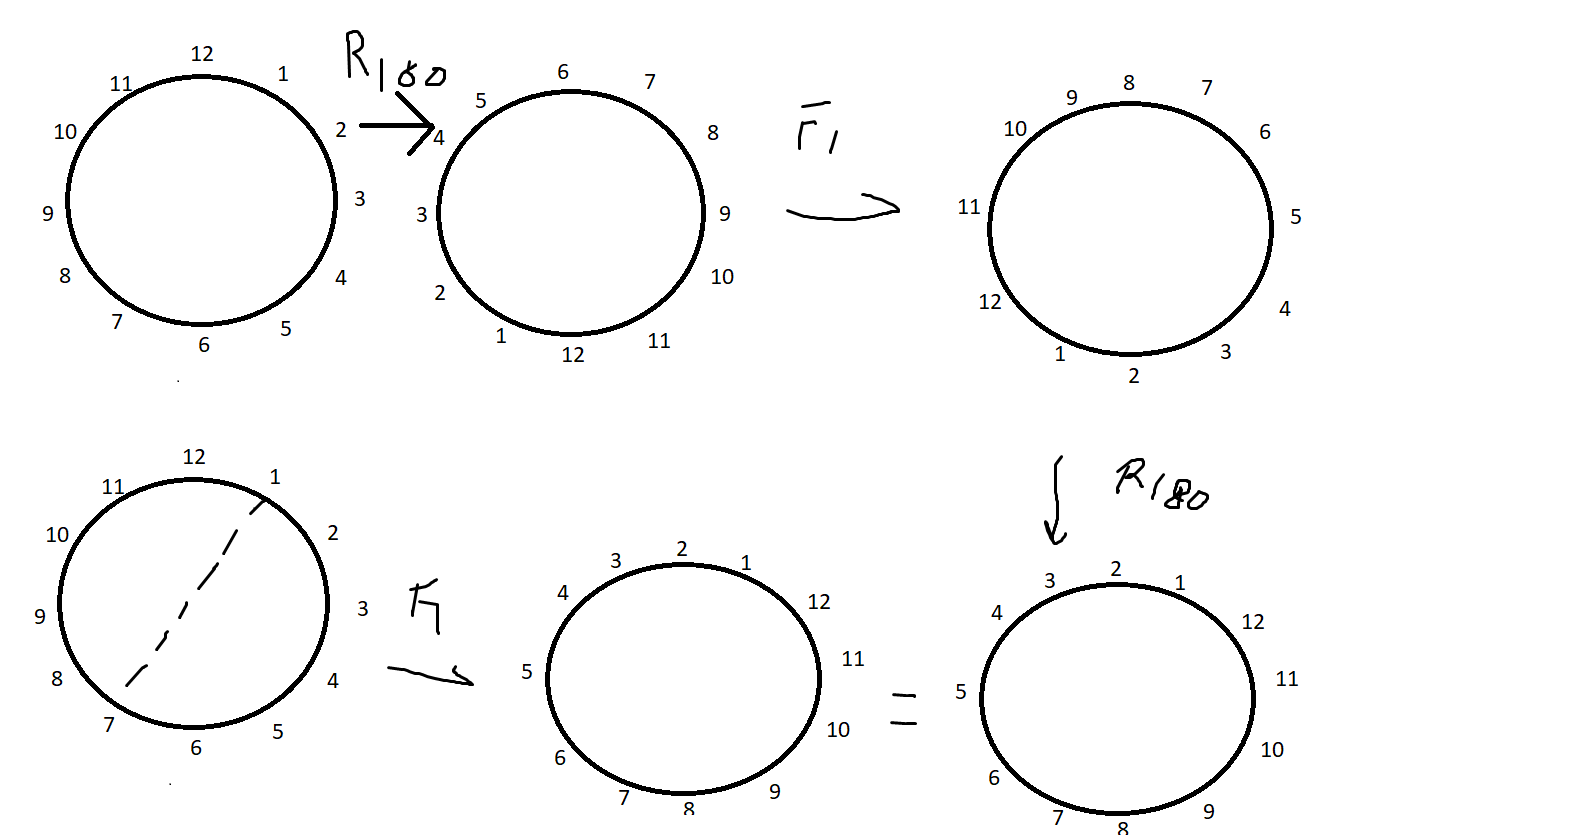
\includegraphics[scale =0.3]{graphically.png}
\\ \\
(c) Yes because rotating 180 degrees clockwise and flipping just makes the next rotation be counterclockwise. This cancels undoes the other rotation just leaving $F_i$
\\ \\
(d) Same reasoning as (c), because rotating 180 degrees clockwise and flipping just makes the next rotation be counterclockwise. This cancels undoes the other rotation just leaving $E_i$

\end{problem}

\begin{problem}{4}
Prove that an abelian group $G$ with two elements $a$ and $b$ of order 2 must have a subgroup $H$ of order 4.
\\ \\
If $G$ is an abelian group with 2 elements $a,b$ with order 2, then $a^2,b^2=e$. Since $a*a = e$ and $b*b=e$, $a^{-1}=a$ and $b^{-1}=b$. It follows that $a*b*a*b = a*a*b*b = e*e = e$ so $a*b^{-1} = a*b$ and $e^{-1} = e$. If I let $H = \langle \left\{e,a,b,a*b \right\}, * \rangle$, every element in $H$ has an inverse and $H$ is closed. I can show $H$ is closed by showing all operations by left multiplication because it is an abelian group, commutativity holds. They are $e*e = e, e*a = a, e*b=b, e*(a*b)=a*a=e, a*b=a*b, a*(a*b) = e*b=b, b*b=e, b*(a*b) = b*b*a = a.$ This shows $H$ is closed. Since $H$ is closed under the binary operation of $G$ and for all $a \in H$, $a^{-1}$ exists, by Corollary 4.2.2 $H$ is a subgroup of $G$.
\end{problem}

\begin{problem}{5}
Consider $U_{18}$, the group of all the 18th roots of unity.
\begin{itemize}
\item[(a)] List the elements of $U_{18}$ in the form of $\omega^k$ for some fixed complex number $\omega$. What should be your choice for $\omega$? In other words, which complex number should $\omega$ be?
\item[(b)] Let $S=\{1,\omega^3,\omega^6,\omega^9,\omega^{12},\omega^{15}\}$. Show that $S \leq U_{18}$.
\item[(c)] Let $T = \{1,\omega^6,\omega^{12}\}.$ Show that $T\leq S$.
\end{itemize}
\hrulefill \\
(a) $U_{18}$ = $\{1,\omega ,\omega^2,\omega^3,\omega^4,\omega^5,\omega^6,\omega^7,\omega^8,\omega^9,\omega^{10},\omega^{11},\omega^{12},\omega^{13},\omega^{14},\omega^{15},\omega^{16},\omega^{17}\}$, and $\omega = \text{cis}(\frac{360}{18}) = \text{cis}(20)$
 \\ \\
(b)\\ $\begin{array}{c|c|c|c|c|c|c}
* & 1 & \omega^{3} & \omega^{6} & \omega^{9} & \omega^{12} & \omega^{15}\\\hline
1 & 1 & \omega^{3} & \omega^{6} & \omega^{9} & \omega^{12} & \omega^{15}\\\hline
\omega^{3} &\omega^{3}& \omega^{6} & \omega^{9} & \omega^{12} & \omega^{15} & 1 \\\hline
\omega^{6} & \omega^{6} & \omega^{9} & \omega^{12} & \omega^{15} & 1 & \omega^{3} \\\hline
\omega^{9} & \omega^{9 }& \omega^{12} & \omega^{15} & 1 & \omega^{3} & \omega^{6} \\\hline
\omega^{12} &\omega^{12} &\omega^{15} & 1 & \omega^{3} & \omega^{6} & \omega^{9} \\\hline
\omega^{15} & \omega^{15} & 1 & \omega^{3} & \omega^{6} & \omega^{9} & \omega^{12} \\\hline
 \end{array}$ \\ \\
Since $\forall a,b \in S$, $a*b \in S$ as shown above, is closed. Now to show $\forall a \in S, a^{-1} \in S$, I show there is an $a^{-1}$ such that $a*a^{-1} = e$. This is when $a^-1 = \omega^{18-k}$ where $a=\omega^k$. Using Corollary 4.2.2, this proves $S\leq U_{18}$
\\ \\
(c) 
$\begin{array}{c|c|c|c}
* & 1& \omega^{6}& \omega^{12} \\\hline
1 & 1 & \omega^{6} & \omega^{12} \\\hline
\omega^{6} & \omega^{6} & \omega^{12} & 1 \\\hline
\omega^{12} & \omega^{12} & 1 & \omega^{6} \\\hline
\end{array}$ \\ \\
Since $\forall a,b \in T$, $a*b \in T$ is closed. Now to show $\forall a \in T, a^{-1} \in T$, I show there is an $a^{-1}$ such that $a*a^{-1} = e$. This is when $a^-1 = \omega^{18-k}$ where $a=\omega^k$. Using Corollary 4.2.2, this proves $T\leq U_{18}$
\end{problem}

\begin{problem}{6}
Let $H=\{a+bi \ | \ a,b \in \mathbb{R} \ \text{and} \ a^2+b^2 = 1\}$. Describe the elements of $H$ geometrically. Prove or disprove that $H$ is a subgroup of $\mathbb{C}^*$ under multiplication. 
\\ \\
$H$ represents the unit complex circle.
$H$ is a subgroup of $\mathbb{C}^*$ under multiplication because it satasfies all requirements of Corollary 4.2.3. First, $\forall a,b\in \mathbb{C}^* $, $b^{-1}$ exists because I can find an element $b^{-1}$ such that $bb^{-1} = 1+1i$. If $b=c+di$, $b^{-1} = \frac{1}{c} + \frac{1}{d}i$ and if I let $e=\frac{1}{c}$ and $f = \frac{1}{d}$, then $b^{-1} = e+fi$. To show that $ab^{-1} \in H$, I will multiply them out and show that the real part squared plus the coeficcient of the imaginary part squared is equal to one. That is, if $a=(x+yi)$ and $b^{-1} = e+fi$ then,
$$ab^{-1} = (x+yi)(e+fi) = -xe -xfi -yei + yf = -xe + yf + (-xf - ye)i$$ and to show
$$(-xe + yf)^2 + (-xfi - yei)^2 = 1$$ I simplify further to find
$$(-xe + yf)^2 = (xe)^2 -2xeyf + (yf)^2  $$
and
$$ (-xfi - yei)^2= (xf)^2 + 2xfye + (ye)^2$$
adding these two together I get
$$(xe)^2 +  (xf)^2 + (yf)^2 +(ye)^2 = x^2(e^2 +f^2) + y^2(e^2+f^2) = x^2(1) + y^2(1) = x^2+y^2 = 1 $$
This shows that $ab^{-1} \in H$. Since $ab^{-1} \in H$ and $H$ is nonempty because $ab^{-1}$ exists, by Corollary 4.2.3, $H$ is a subgroup of $\mathbb{C}^*$ under multiplication. 
\end{problem}
\begin{problem}{7}
Prove that if $G$ is an abelian group with identity $e$, then all elemennts $x$ of $G$ satisfying the equation $x^2 = e$ form a subgroup of $G$. Be sure to show all the steps in your argument.
\\ \\
I want to show that $H = \{x\in G \ | \ x^2=e\} \leq G$. To do this I will use Corollary 4.2.3.
$H$ is nonempty because it contains $e$. $b^{-1}=b$ because $b^2 = b*b= e$. Then, $a*b^{-1} \in H$ because $(a*b^{-1})^2 = (a*b)^2 = a*a*b*b= e*e = e $ which also means $(a*b)^{-1} = a*b$. Since $H$ is nonempty and $ab^{-1}$ exists for all $a,b\in H$, then by Corollary 4.2.3, $H$ is a subgroup of $G$.
\end{problem}

\begin{problem}{8}
Let $p$ and $q$ be distinct primes. Suppose $H < \mathbb{Z}$ and $H$ contains $exactly$ three of the five elements $p, p+q, pq, p^q, $ and $q^p$. Determine which of the following are these three elements.
\\ \\ 
The answer is $(iii)\  p, p+q, pq$
\end{problem}

\begin{problem}{9}
List the elements of $\langle\frac{1}{2}\rangle$ in $\langle \mathbb{Q}, + \rangle$ and in $\langle \mathbb{Q}^*, \cdot \rangle$. 
\\
\\
The elements that $\langle Q, + \rangle $ and $\langle Q^*, \cdot \rangle$ share is equal to $\{ 2^n \ | \ n \geq -1\ , n \in \mathbb{Z}\}$
\end{problem}

\begin{problem}{10}
Recall that $U(20) = \mathbb{Z}^*_{20}$. What are its elements? How can you check whether $U(20)$ is cyclic? \\ \\
The elements are $$ U(20) = \{7,9,11,13,17,19\}$$
I could check to see whether $U(20)$ is cyclic by checking if there is a generator in $U(20)$ that generates $U(20)$. If there is, it is cyclic, but if there isn't it is not.

\end{problem}

\begin{problem}{11}
The group $U(15)$ has six cyclic subgroups. List them.
\\ \\
The cyclic subgroups of $U(15)$ are
\begin{align*}
\langle 1 \rangle &= \{1\} \\
 \langle 2 \rangle &= \{2,4,8,1\}\\
 \langle 4 \rangle &= \{4,1\}\\
\langle 7 \rangle &= \{7,4,13,1\}\\
\langle 11 \rangle &= \{11,1\} \\
\langle 14 \rangle &= \{14,1\}\\
\end{align*}
\end{problem}
\end{document}
